\section{HIDDEN MARKOV MODEL PREDICTION}
\label{sec:hmm}
We can try a different method to predict the future of an economy. We can study the economies as a Markov Chain, a stochastic model describing a sequence of possible events in which the probability of each event depends only on the state attained in the previous event.

Our new approach involves incorporating three variables into a Hidden Markov Model. This version is designed to estimate the probabilities of transitioning from one state to another, relying not on direct knowledge of these probabilities but on observations of a related variable. To achieve this, we defined four basic states based on the possible increases and decreases in the Interest Rate and Consumer Price Index. Additionally, we considered two observable variables: the increase and decrease of GDP.

We will make some assumptions on the economic data, considering them dependent only on the previous point and not on the full sequence before them, and limiting the states only on positive or negative increases. The first assumption simplifies our work and allows us to use a Markov Chain, even if of course the complex relation of real economy figures is not so simple; the second does not capture the full spectrum of possibilities but allows us to more easily make consideration on the result, having only four states and two known variables. In the future, dividing the data into multiple steps could result in a better model that is able to differentiate between good and extreme differences: inflation at 3\% versus 80\% like in Türkiye; increasing the interest rate from a base of -0.5\% versus from 4.5\%; a good increase of 4\% of GDP versus a 0.2\% increase that saves a country for being in a technical recession. For the scope of this paper, however, we will stick to the simpler version.

To create our model, we used the Baum-Welch Algorithm \cite{baum}. This algorithm is an iterative procedure that estimates the parameters of a Hidden Markov Model. We start with a Hidden Markov Chain and a known variable chain created from the statistics of one starting country and then we use the temporal series of all the country we have to improve our model over multiple iterations.

Based on the data available, we ended up using twenty-five countries: Brazil, Canada, Chile, Denmark, Finland, France, Germany, Greece, Ireland, India, Indonesia, Italy, Israel, Japan, Mexico, Netherlands, Norway, Russia, South Africa, Spain, Switzerland, South Korea, Ukraine, United Kingdom, United States. We divided the data so that recent measurements between 2017 and 2020 were used for testing, while after 2020 we make some considerations about the recent crisis. Not all countries used for training, however, have data available for the testing or COVID analysis, but they are still useful for the model iterations.

\subsection*{Baum Welch Algorithm}
We start by creating a starting HMM model by calculating the probabilities from the starting country based on its data. We can define

\begin{itemize}
    \item $X_t$ as the hidden state at time $t$ (which can be a combination of increase/decrease of interest rate/consumer price index)
    \item $Y_t$ as the country observation temporal series of the known variable at time $t$ (which can be the increase or decrease of the GDP)
    \item $ A= \{a_{ij}\} = P(X_t = j | X_{t-1} = i)$ as the transition matrix between the hidden chain states
    \item $B = \{b_j(y_i)\} = P(Y_t = y_i | X_t = j)$ as the observation matrix between a a known variable and hidden state
    \item$\pi$ as the initial hidden state distribution
\end{itemize}
We will call the Hidden Markov chain \(\theta = (A,B,\pi)\).

Then, we iterate for the number of epochs by calculating for each country temporal series the forward ($\alpha$) and backward ($\beta$) probabilities, where

\[\alpha_t(i) = P(Y_1 = y_1, ..., Y_t = y_t, X_t = i | \theta)\]

are the probabilities of seeing the observations $y_1, ..., y_t$ and being in state $i$ at time $t$, calculated as

\[\alpha_i(1) = \pi_i b_i(y_1)\]
\[\alpha_i(t+1) = b_i(y_{t+1}) \sum_{j=1}^{N} \alpha_j(t) a_{ji}\]

and

\[\beta_t(i) = P(Y_{t+1} = y_{t+1}, ..., Y_T = y_T | X_t = i, \theta)\]

are the probabilities of the ending partial sequence $y_{t+1}, ..., y_T$ given starting state $i$ at time $t$, calculated as

\[\beta_i(T) = 1\]
\[\beta_i(t) = \sum_{j=1}^{N} a_{ij} b_j(y_{t+1}) \beta_j(t+1)\]

We can calculate the temporary variables

\[\gamma_t(i) = P(X_t = i | Y, \theta) = \frac{\alpha_i(t)\beta_i(t)}{\sum_{j=1}^{N} \alpha_j(t) \beta_j(t)}\]

being the probability of being in state $i$ at time $t$

\[\xi_t(i, j) = P(X_t = i, X_{t+1} = j | Y, \theta) =\]

\[\frac{\alpha_i(t) a_{ij} \beta_j(t+1) b_j(y_t+1)}{\sum_{k=1}^{N}\sum_{w=1}^{N}\alpha_k(t) a_{kw} \beta_w(t+1) b_w(y_t+1)}\]

being the probability of transitioning from state $i$ to state $j$ at time $t$

If we calculate $(\alpha_r, \beta_r, \gamma_r, \xi_r)$ $\forall r \in R \text{ countries }$, we can use all of them to update the parameters of $\theta$

\[\pi_i = \sum_{r=1}^{R} \gamma_{ir}(1)\]

\[a_{ij} = \frac{\sum_{r=1}^{R} \sum_{t=1}^{T-1} \xi_{ijr}(t)}{\sum_{r=1}^{R} \sum_{t=1}^{T-1} \gamma_{ir}(t)}\]

\[b_i(v_k) = \frac{\sum_{r=1}^{R} \sum_{t=1}^{T} 1_{y_{tr} \ne v_k} \gamma_{ir}(t)}{\sum_{r=1}^{R} \sum_{t=1}^{T} \gamma_{ir}(t)}\]

\[\text{where } 1_{y_{tr} \ne v_k} = \begin{cases} 1 & \text{if $y_{tr} \ne v_k$} \\ 0 & \text{otherwise} \end{cases}\]

\subsection*{Results}

By having now a model that can estimate the probabilities of transitioning from one state to another, we can use it to predict the future of a country. We must first test the model working on real data: to do that, we use the model trained on data until the end of 2016 and test it on data by making a thousand random walks and comparing results from the start of 2017 to the end of 2019. We can then do the same, only this time with the covid data from the start of 2020 onward to see if the model deviates and how much. Here we show some results on some countries, Italy and United States.

% substitute ± with (@$\pm$@)

\subsubsection*{Italy}

We can see here that the model is able to predict the future of Italy quite well, with the average of the known states being very close to the actual data. For the covid data, the real performance is a bit lower (27 versus predicted 32.37): even if it is inside the prediction interval, we can see how much the recent crisis have impacted the economy.

\begin{figure}[H]
    \centering
    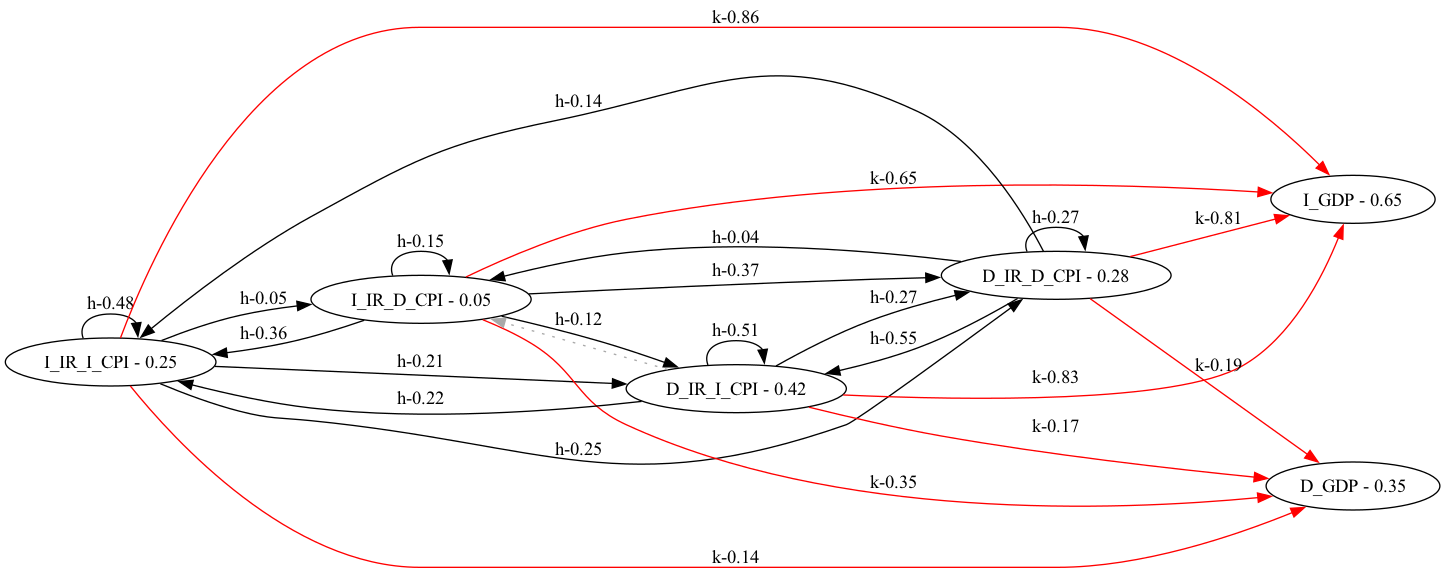
\includegraphics[width=\columnwidth]{imgs/italy_hmm.png}
    \caption{Hidden Markov Chain for Italy}
    \label{fig:correlation_us}
\end{figure}

\begin{table}[H]
  \centering
  \begin{tabular}{|c|c|c|c|}
    \hline
    State         & Ground Truth & Prediction & PI     \\
    \hline
    I\_IR\_I\_CPI & 8            & 9.95       & ± 7.20 \\
    I\_IR\_D\_CPI & 2            & 1.02       & ± 2.19 \\
    D\_IR\_I\_CPI & 11           & 15.57      & ± 7.21 \\
    D\_IR\_D\_CPI & 15           & 9.46       & ± 5.26 \\
    I\_GDP        & 30           & 29.85      & ± 4.38 \\
    D\_GDP        & 6            & 6.15       & ± 4.38 \\
    \hline
  \end{tabular}
  \label{tab:italy_test}
  \caption{Hidden Markov Model predictions for test set of Italy}
\end{table}

\begin{table}[H]
  \centering
  \begin{tabular}{|c|c|c|c|}
    \hline
    State         & Ground Truth & Prediction & PI     \\
    \hline
    I\_IR\_I\_CPI & 13           & 10.80      & ± 6.99 \\
    I\_IR\_D\_CPI & 3            & 1.11       & ± 2.29 \\
    D\_IR\_I\_CPI & 14           & 16.75      & ± 7.12 \\
    D\_IR\_D\_CPI & 9            & 10.34      & ± 5.54 \\
    I\_GDP        & 27           & 32.37      & ± 4.49 \\
    D\_GDP        & 12           & 6.63       & ± 4.49 \\
    \hline
  \end{tabular}
  \label{tab:italy_covid}
  \caption{Hidden Markov Model predictions for covid data of Italy}
\end{table}

\subsubsection*{United States}

The United States, like before, are quite the outliers: since the model is trained on all countries even if the USA have not experienced a single month of negative GDP growth, the prediction is a bit more pessimistic (even if it is still inside our prediction interval). The situation during the COVID pandemic changes things: during this negative period, the USA mighty performance is similar to a normal country before the crisis.

\begin{figure}[H]
    \centering
    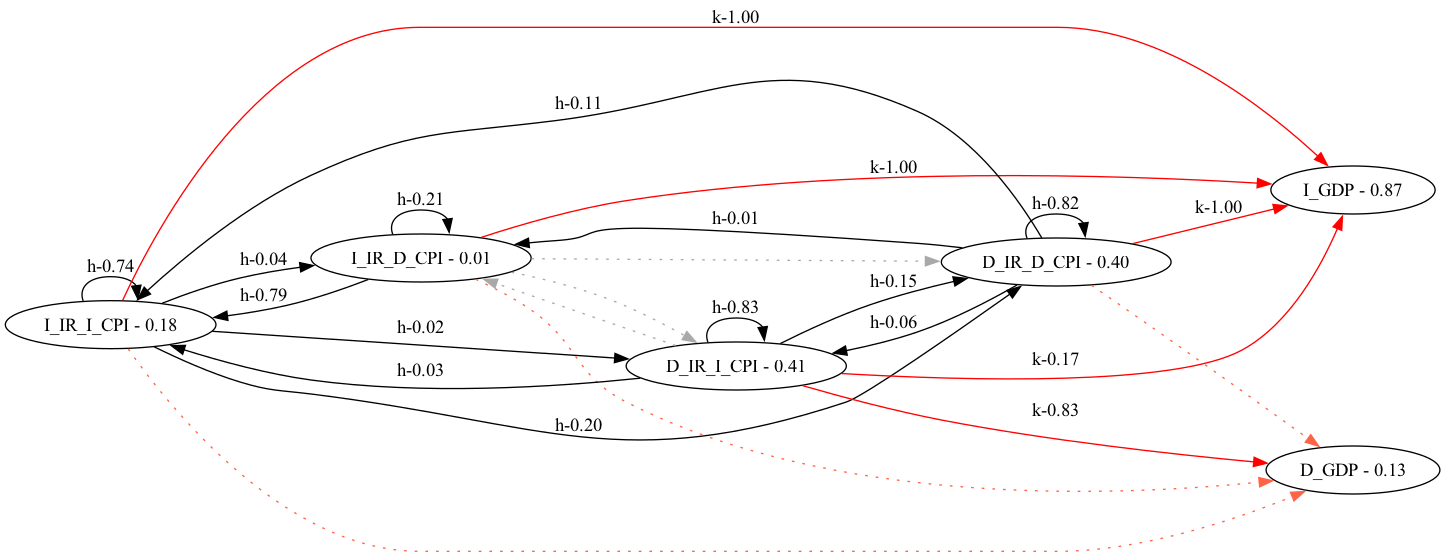
\includegraphics[width=\linewidth]{imgs/usa_hmm.png}
    \caption{Hidden Markov Chain for USA}
    \label{fig:correlation_us}
\end{figure}

\begin{table}[H]
  \centering
  \begin{tabular}{|c|c|c|c|}
    \hline
    State         & Ground Truth & Prediction & PI      \\
    \hline
    I\_IR\_I\_CPI & 10           & 10.47      & ± 11.57 \\
    I\_IR\_D\_CPI & 2            & 0.75       & ± 2.21  \\
    D\_IR\_I\_CPI & 2            & 7.23       & ± 12.30 \\
    D\_IR\_D\_CPI & 22           & 17.55      & ± 12.40 \\
    I\_GDP        & 36           & 29.93      & ± 10.34 \\
    D\_GDP        & 0            & 6.07       & ± 10.34 \\
    \hline
  \end{tabular}
  \label{tab:usa_test}
  \caption{Hidden Markov Model predictions for test set for USA}
\end{table}

\begin{table}[H]
  \centering
  \begin{tabular}{|c|c|c|c|}
    \hline
    State         & Ground Truth & Prediction & PI     \\
    \hline
    I\_IR\_I\_CPI & 0            & 5.93       & ± 8.63 \\
    I\_IR\_D\_CPI & 0            & 0.40       & ± 1.58 \\
    D\_IR\_I\_CPI & 0            & 3.73       & ± 8.66 \\
    D\_IR\_D\_CPI & 20           & 9.95       & ± 9.10 \\
    I\_GDP        & 14           & 16.85      & ± 7.37 \\
    D\_GDP        & 6            & 3.15       & ± 7.37 \\
    \hline
  \end{tabular}
  \label{tab:usa_covid}
  \caption{Hidden Markov Model predictions for covid data for USA}
\end{table}

\subsubsection*{South Korea}
With South Korea the testing of our prediction is well acceptable. The test on the covid data however is also quite similar: the republic of Korea had an excellent mechanism of contact tracing and random tests on the population, resulting in a better management of the pandemic, suffered much less than other countries and that resulted in an economy that was not as damaged as the others.

\begin{figure}[H]
    \centering
    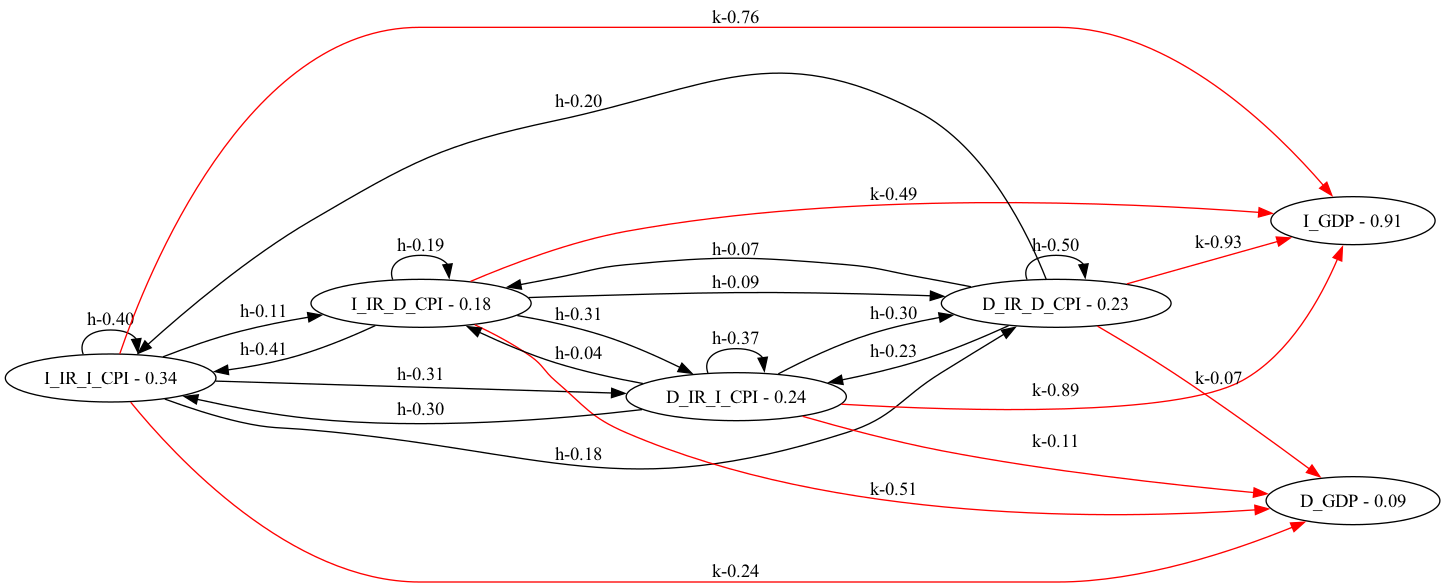
\includegraphics[width=\linewidth]{imgs/sk_hmm.png}
    \caption{Hidden Markov Chain for South Korea}
    \label{fig:correlation_sk}
\end{figure}

\begin{table}[H]
  \centering
  \begin{tabular}{|c|c|c|c|}
    \hline
    State         & Ground Truth & Prediction & PI      \\
    \hline
    I\_IR\_I\_CPI & 8           & 11.07 & ± 6.19 \\
    I\_IR\_D\_CPI & 6            & 2.98 & ± 3.59  \\
    D\_IR\_I\_CPI & 11            & 11.07 & ± 5.93 \\
    D\_IR\_D\_CPI & 11          & 10.88 & ± 7.01 \\
    I\_GDP        & 30           & 29.86 & ± 4.42 \\
    D\_GDP        & 6            & 6.14 & ± 4.42 \\
    \hline
  \end{tabular}
  \label{tab:sk_test}
  \caption{Hidden Markov Model predictions for test set for South Korea}
\end{table}

\begin{table}[H]
  \centering
  \begin{tabular}{|c|c|c|c|}
    \hline
    State         & Ground Truth & Prediction & PI     \\
    \hline
    I\_IR\_I\_CPI & 17            & 12.01 & ± 6.54 \\
    I\_IR\_D\_CPI & 4            & 3.22 & ± 3.93 \\
    D\_IR\_I\_CPI & 12            & 11.87 & ± 6.2 \\
    D\_IR\_D\_CPI & 6           & 11.90 & ± 7.40 \\
    I\_GDP        & 30           & 32.41 & ± 4.80 \\
    D\_GDP        & 9            & 6.58 & ± 4.80 \\
    \hline
  \end{tabular}
  \label{tab:sk_covid}
  \caption{Hidden Markov Model predictions for covid data for South Korea}
\end{table}

\subsubsection*{Model degeneration}
To train the HMM, we used 3 epochs: each time we improved our model on all temporal series, and then repeat. What would happen if we increased a lot the number of epochs? Let's try with 25 epochs.

\begin{figure}[H]
    \centering
    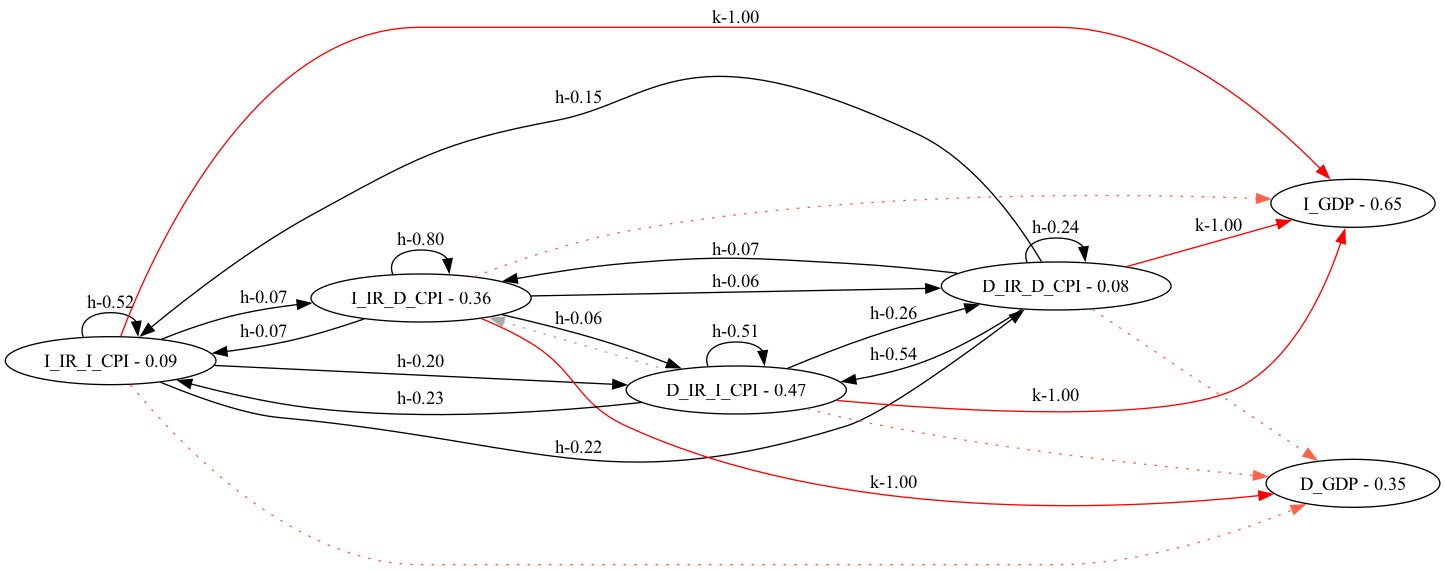
\includegraphics[width=\columnwidth]{imgs/italy_hmm_degenerated.png}
    \caption{Hidden Markov Chain for Italy (degenerated)}
    \label{fig:correlation_us}
\end{figure}

% \begin{lstlisting}
%   ITALY training data has 162 positive and 87 negative values for GDP ([ 66.00  8.00  108.00  67.00])

%   Use test data
%   ITALY testing data has 30 positive and 6 negative values for GDP ([ 8.00  2.00  11.00  15.00])

%   ITALY random walks has produced on average ['9.41 (@$\pm$@) 7.44', '6.09 (@$\pm$@) 11.39', '12.95 (@$\pm$@) 8.43', '7.55 (@$\pm$@) 5.48'] for the hidden states and ['29.91 (@$\pm$@) 11.39', '6.09 (@$\pm$@) 11.39'] for the known states
%   On average we have predicted 29.91 (@$\pm$@) 11.39 positive and 6.09 (@$\pm$@) 11.39 negative values for GDP

%   Use covid data
%   ITALY covid data has 27 positive and 12 negative values for GDP ([ 13.00  3.00  14.00  9.00])

%   ITALY random walks has produced on average ['10.53 (@$\pm$@) 7.86', '6.16 (@$\pm$@) 11.46', '14.11 (@$\pm$@) 8.96', '8.20 (@$\pm$@) 5.59'] for the hidden states and ['32.84 (@$\pm$@) 11.46', '6.16 (@$\pm$@) 11.46'] for the known states
%   On average we have predicted 32.84 (@$\pm$@) 11.46 positive and 6.16 (@$\pm$@) 11.46 negative values for GDP
% \end{lstlisting}
\begin{table}[H]
  \centering
  \begin{tabular}{|c|c|c|c|}
    \hline
    State         & Ground Truth & Prediction & PI      \\
    \hline
    I\_IR\_I\_CPI & 8            & 9.41       & ± 7.44  \\
    I\_IR\_D\_CPI & 2            & 6.09       & ± 11.39 \\
    D\_IR\_I\_CPI & 11           & 12.95      & ± 8.43  \\
    D\_IR\_D\_CPI & 15           & 7.55       & ± 5.48  \\
    I\_GDP        & 30           & 29.91      & ± 11.39 \\
    D\_GDP        & 6            & 6.09       & ± 11.39 \\
    \hline
  \end{tabular}
  \label{tab:italy_test_degen}
  \caption{Hidden Markov Model predictions for test set for Italy (more epochs)}
\end{table}

\begin{table}[H]
  \centering
  \begin{tabular}{|c|c|c|c|}
    \hline
    State         & Ground Truth & Prediction & PI      \\
    \hline
    I\_IR\_I\_CPI & 13           & 10.53      & ± 7.86  \\
    I\_IR\_D\_CPI & 3            & 6.16       & ± 11.46 \\
    D\_IR\_I\_CPI & 14           & 14.11      & ± 8.96  \\
    D\_IR\_D\_CPI & 9            & 8.20       & ± 5.59  \\
    I\_GDP        & 27           & 32.84      & ± 11.46 \\
    D\_GDP        & 12           & 6.16       & ± 11.46 \\
    \hline
  \end{tabular}
  \label{tab:italy_covid_degen}
  \caption{Hidden Markov Model predictions for covid data of Italy (more epochs)}
\end{table}
We can see how our prediction is still working. We have the same mean but larger prediction intervals: each random walk weights more now. The model has degenerated: each hidden state goes only to one known state. Since the testing still works, we could say that this Markov Chain is showing us a correlation. All states but I\_IR\_D\_CPI increases the GDP: an increase in the interest rate and a decrease in the inflation instead decreases it. This result is in line with our initial assumptions, although simplified.

We can also see some missing links that are quite logical, like from I\_IR\_D\_CPI to D\_IR\_I\_CPI, and most states but D\_IR\_D\_CPI tend to remain in the same state. This also makes sense: if the inflation is decreasing and we decrease the interest rate, the inflation is going to go up since people will start borrowing money more frequently.
